\documentclass[12pt]{article}

\input preamble

\title{Principles of Parallel Architecture\\
Amdahl’s law and speed up}
\author{Xitong Liu \\
xliu@ece.udel.edu}

\begin{document}

\maketitle

\section{Questions}
\begin{enumerate}

\item Serial Matrix Multiplication
\begin{description}
\item[Q:] The first thing you need to do is to implement a C program 
for Matrix Multiplication, serially, for a single processor.

Your implementation will create and initialize 2 matrices of size N 
by N (that are called MatrixA and MatrixB) and multiply them (Store 
the result in a variable called MatrixC).

The value of N will be given to your program through the command line. 
The value of each element of the Matrices will be random double 
precision numbers from -1 to 1.

Also, for testing purposes, if N is less than 6, the program will 
automatically print to the screen matrices MatrixA, MatrixB and 
MatrixC.
\item[A:] 
Source Code:
\footnotesize
\begin{verbatim}
#include <stdio.h>
#include <stdlib.h>
#include <string.h>
#include <unistd.h>
#include <sys/time.h>

//global varialbes and definitions
#define OUTPUT_THRESHOLD 6

char * usage = "Usage: mm N\n";
char * matrix_size_error = "Invalid matrix size N = %d.
  It must be greater than 1.\n";
char * matrix_size_info = "Matrix Size N = %d\n";
char * malloc_error = "Malloc ERROR.\n";

void print_matrix(double * matrix, int matrixSize);

int main( int argc, char *argv[] )
{
  int matrixSize = 0;
  double * matrixA = NULL;
  double * matrixB = NULL;
  double * matrixC = NULL;
  
  struct timeval tv;
  struct timeval __start;
  struct timeval  __end;
  double t_start = 0.0f;
  double t_end = 0.0f;
  double Ti = 0.0f;
  double Tc = 0.0f;
  double Tt = 0.0f;

  int cycleI = 0;
  int cycleJ = 0;
  int cycleK = 0;

  if(argc < 2){
    puts(usage);
    exit(-1);
  }

  // get the matrix from the command line options list
  matrixSize = atoi(argv[1]);
  if(1 > matrixSize){
    printf(matrix_size_error, matrixSize);
    exit(-1);
  }
  printf(matrix_size_info, matrixSize);

  if(NULL == (matrixA = malloc( matrixSize * matrixSize * sizeof(double)))){
    puts(malloc_error);
    exit(-1);
  }
  if(NULL == (matrixB = malloc( matrixSize * matrixSize * sizeof(double)))){
    puts(malloc_error);
    free(matrixA);
    exit(-1);
  }
  if(NULL == (matrixC = malloc( matrixSize * matrixSize * sizeof(double)))){
    puts(malloc_error);
    free(matrixA);
    free(matrixB);
    exit(-1);
  }

  //initilize random generator
  gettimeofday(&tv, NULL);
  srand(tv.tv_sec * tv.tv_usec);
  gettimeofday(&__start, NULL);
  // initilize the matrix by random numbers between -1.00f and 1.00f
  for(cycleI = 0; cycleI < matrixSize * matrixSize; ++ cycleI){
    matrixA[cycleI] = (double)rand() / ((double)(RAND_MAX)+ 1.00) * 2.0 - 1.0;
    matrixB[cycleI] = (double)rand() / ((double)(RAND_MAX)+ 1.00) * 2.0 - 1.0;
  }
  gettimeofday(&__end, NULL);
  t_end = (__end.tv_sec + (__end.tv_usec/1000000.0));
  t_start = (__start.tv_sec + (__start.tv_usec/1000000.0));
  Ti = t_end - t_start;
  gettimeofday(&__start, NULL);
  // do the matrix multiplication
  for(cycleI = 0; cycleI < matrixSize; ++ cycleI){
    for(cycleJ = 0; cycleJ < matrixSize; ++ cycleJ){
      matrixC[cycleI * matrixSize + cycleJ] = 0.0f;
      for(cycleK = 0; cycleK < matrixSize; ++ cycleK){
        matrixC[cycleI * matrixSize + cycleJ] += 
          matrixA[cycleI * matrixSize + cycleK] *
          matrixB[cycleK * matrixSize + cycleJ];
      }
    }
  }
  gettimeofday(&__end, NULL);
  t_end = (__end.tv_sec + (__end.tv_usec/1000000.0));
  t_start = (__start.tv_sec + (__start.tv_usec/1000000.0));
  Tc = t_end - t_start;
  Tt = Ti + Tc;
  
  // if the matrix size is below the threshold, output the result
  if(matrixSize < OUTPUT_THRESHOLD){
    printf("MatrixA:\n");
    print_matrix(matrixA, matrixSize);
    printf("MatrixB:\n");
    print_matrix(matrixB, matrixSize);
    printf("MatrixC:\n");
    print_matrix(matrixC, matrixSize);
  }

  free(matrixA);
  free(matrixB);
  free(matrixC);
  printf("Ti: %fs\n", Ti);
  printf("Tc: %fs\n", Tc);
  printf("Tt: %fs\n", Tt);
  return 0;
}

void print_matrix(double * matrix, int matrixSize){
  int cycleI = 0;
  int cycleJ = 0;

  for(cycleI = 0; cycleI < matrixSize; ++ cycleI){
    for(cycleJ = 0; cycleJ < matrixSize; ++ cycleJ){
      if(matrix[cycleI * matrixSize + cycleJ] > 0.0f){
        printf("+%f\t", matrix[cycleI * matrixSize + cycleJ]);
      }else{
        printf("%f\t", matrix[cycleI * matrixSize + cycleJ]);
      }
    }
    printf("\n");
  }
}
\end{verbatim}
\end{description}

\item Parallel Matrix Multiplication
\begin{description}
\item[Q:]
In this case, you will use MPI to parallelize your Matrix 
Multiply application. As before, the names for the matrices 
will be MatrixA, MatrixB and MatrixC. Also, the size of the 
matrices remain NxN and N is a parameter passed through the 
command line.

The number of MPI processes to use is decided when the program 
is launched. For example if you run your program with:

\begin{verbatim}
mpirun �np 7 mpi_matmult 5 
\end{verbatim}

There will be 7 processors working to achieve the multiplication 
of 5x5 matrices. As before, when N is less than 6, automatically 
print the matrices to the screen.
\item[A:]
\end{description}

\end{enumerate}
\end{document}

\begin{comment}
\begin{figure}[h!]
	\begin{center}
		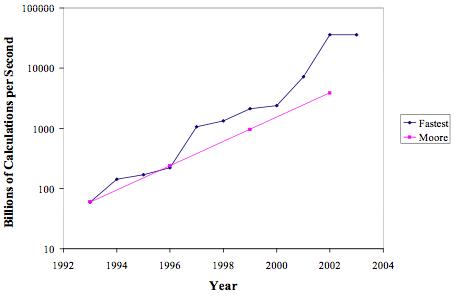
\includegraphics[width=0.7\textwidth, angle=0]{fatest.png}
		\caption{\label{fig:fatest}Fatest SuperComputer in the world}
	\end{center}
\end{figure}
\end{comment}